\section{Results}
 \begin{figure}[t]
	\centering
	\subfigure[A 4-connected tile.] {
	%\vspace{-5em}
		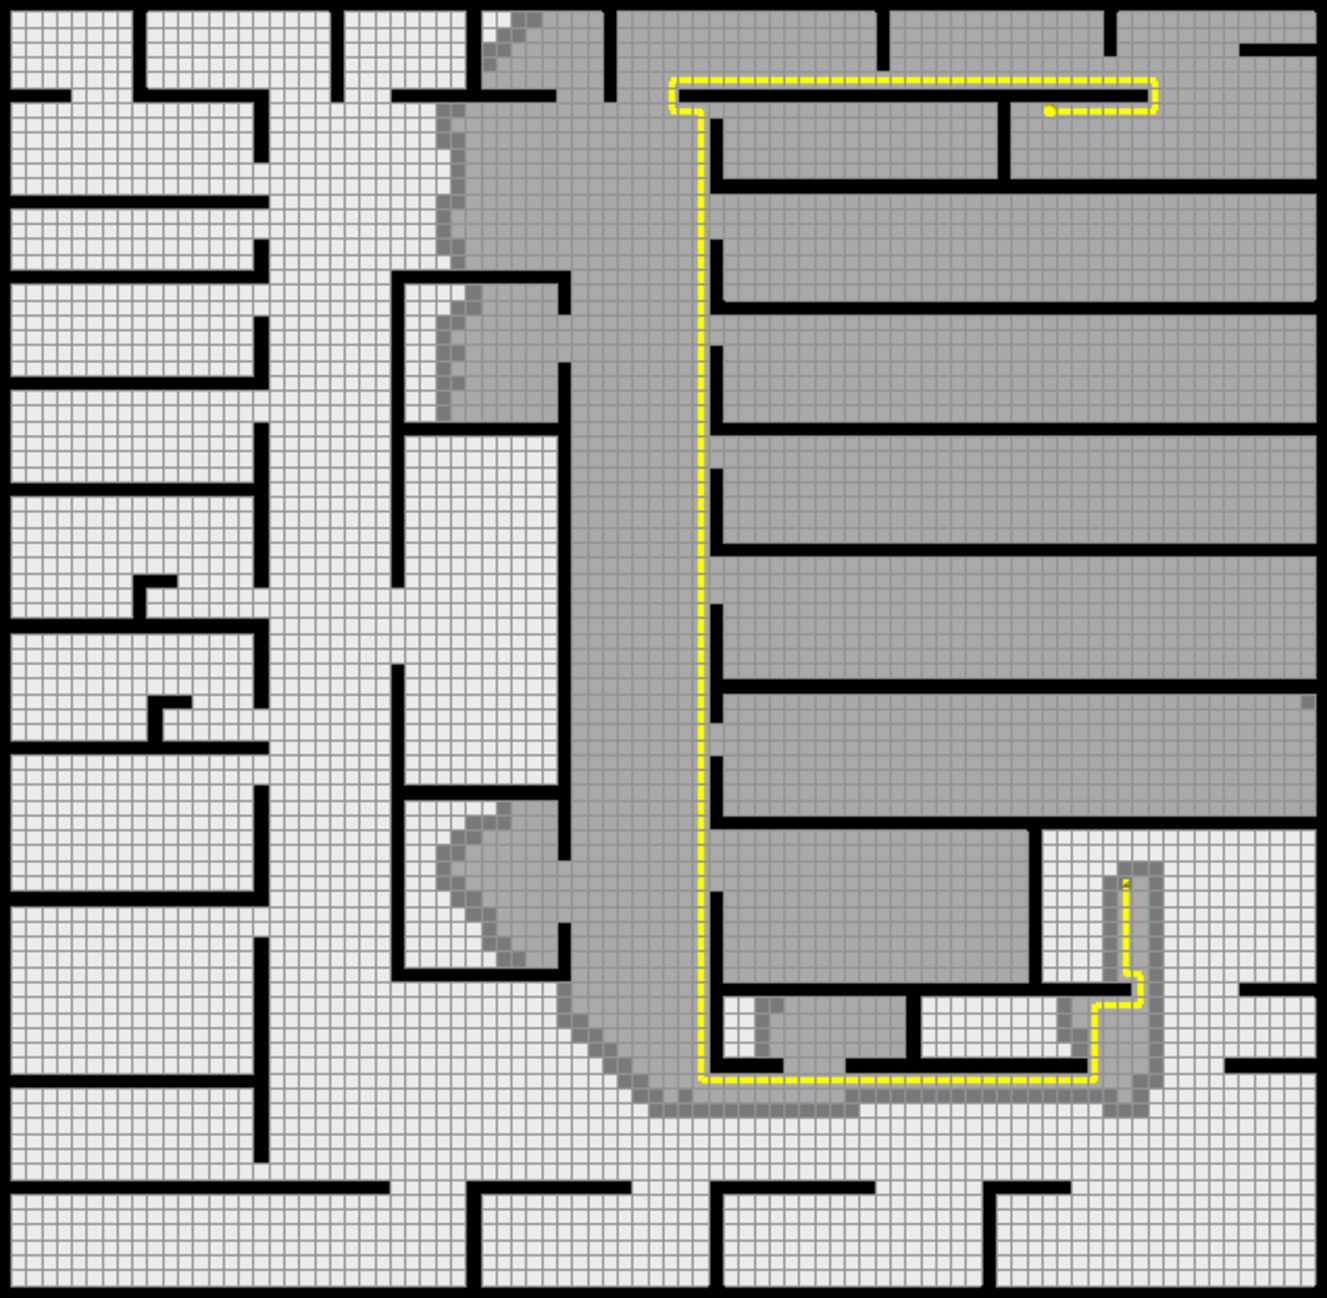
\includegraphics[width=0.47\columnwidth]{diagrams/astarsearch.pdf}
	}
	\subfigure[A 8-connected octile.] {
	%\vspace{-5em}
		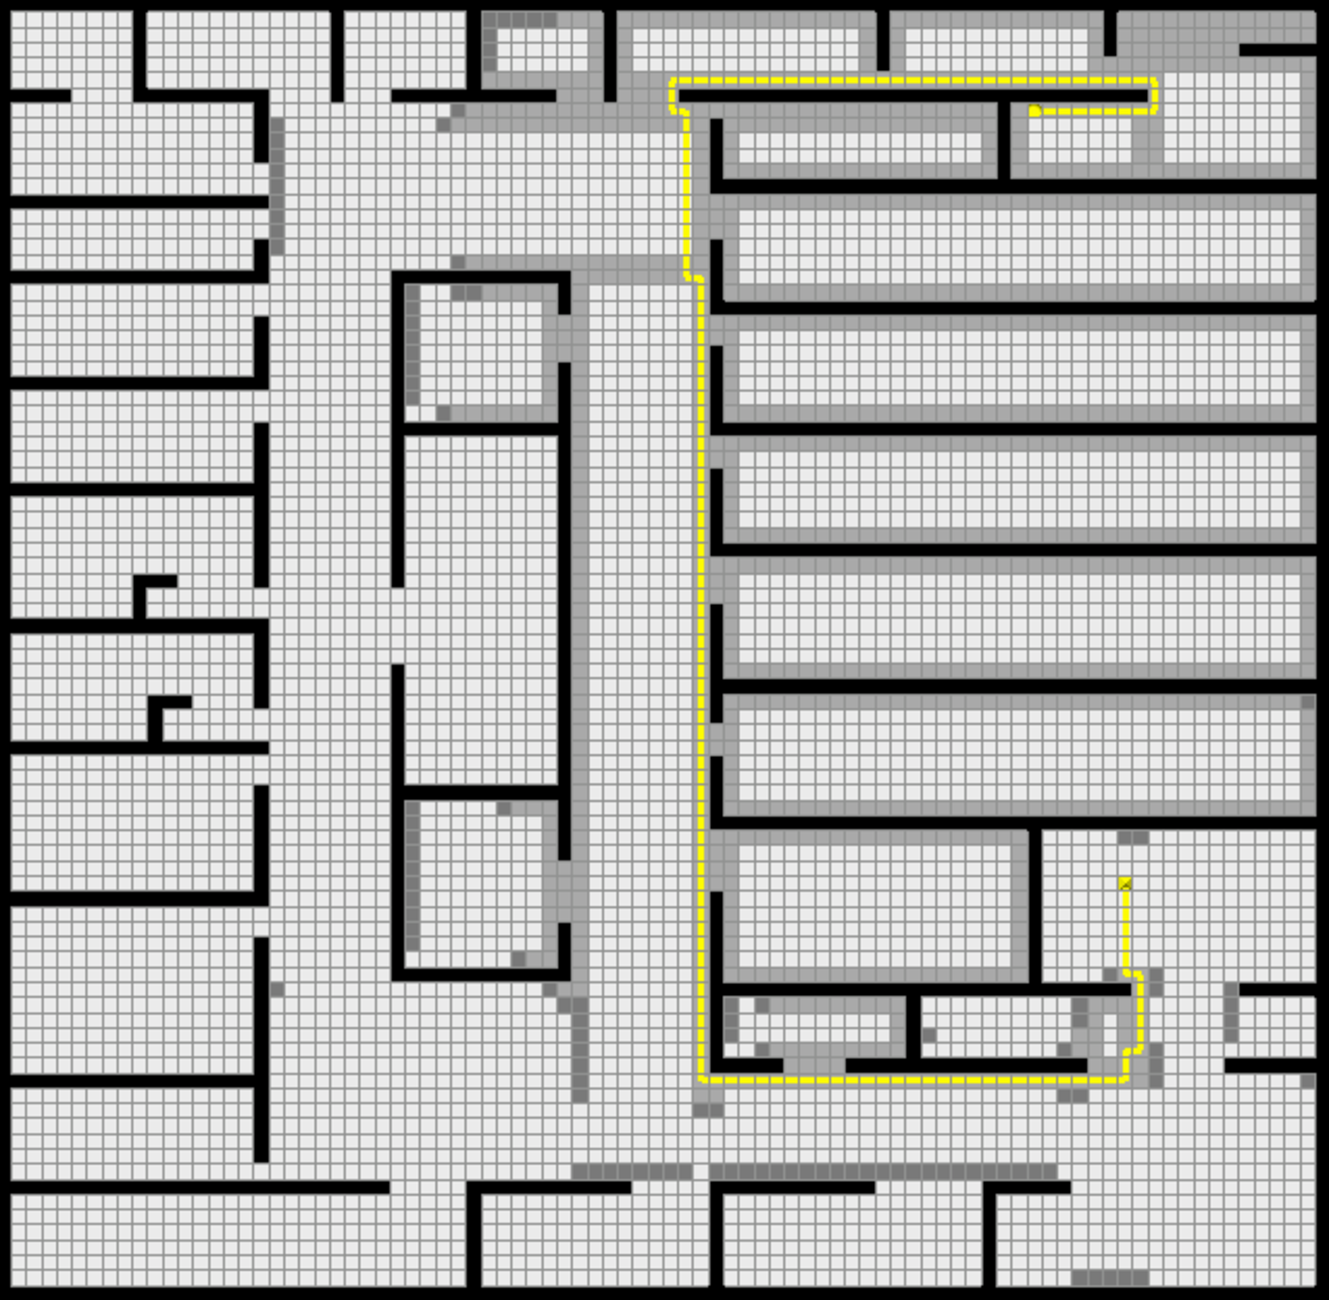
\includegraphics[width=0.47\columnwidth]{diagrams/psearch.pdf}
	}
	\caption{The two most popular types of grid maps are tiles (which have
up to 4 neighbours) and octiles (which have up to 8 neighbours).}
\vspace{1em}
 \end{figure}
% \begin{wrapfigure}{R}{0.39\columnwidth}
%%\vspace{-5.5em}
%		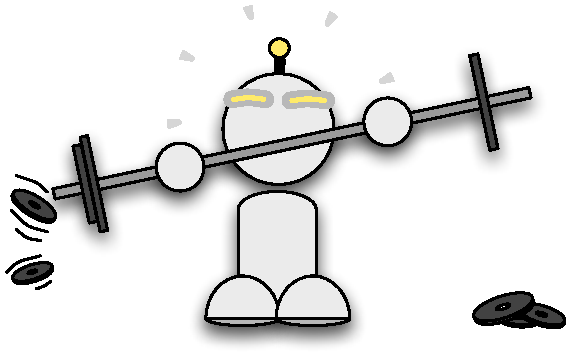
\includegraphics[width=0.39\columnwidth, trim = 10mm 10mm 10mm 10mm]{diagrams/robot_weights.pdf}
% \end{wrapfigure}

Pathfinding is a problem. Blah blah blah.
Lorem ipsum dolor sit amet, consectetur adipisicing elit, sed do eiusmod
tempor incididunt ut labore et dolore magna aliqua. Ut enim ad minim
veniam, quis nostrud exercitation ullamco laboris nisi ut aliquip ex ea
commodo consequat. Duis aute irure dolor in reprehenderit in voluptate
velit esse cillum dolore eu fugiat nulla pariatur. Excepteur sint occaecat
cupidatat non proident, sunt in culpa qui officia deserunt mollit anim
id est laborum.


Pathfinding is a problem. Blah blah blah.
Lorem ipsum dolor sit amet, consectetur adipisicing elit, sed do eiusmod
tempor incididunt ut labore et dolore magna aliqua. Ut enim ad minim
veniam, quis nostrud exercitation ullamco laboris nisi ut aliquip ex ea
commodo consequat. Duis aute irure dolor in reprehenderit in voluptate
velit esse cillum dolore eu fugiat nulla pariatur. Excepteur sint occaecat
cupidatat non proident, sunt in culpa qui officia deserunt mollit anim
id est laborum.

\begin{figure}[t]
\begin{center}
		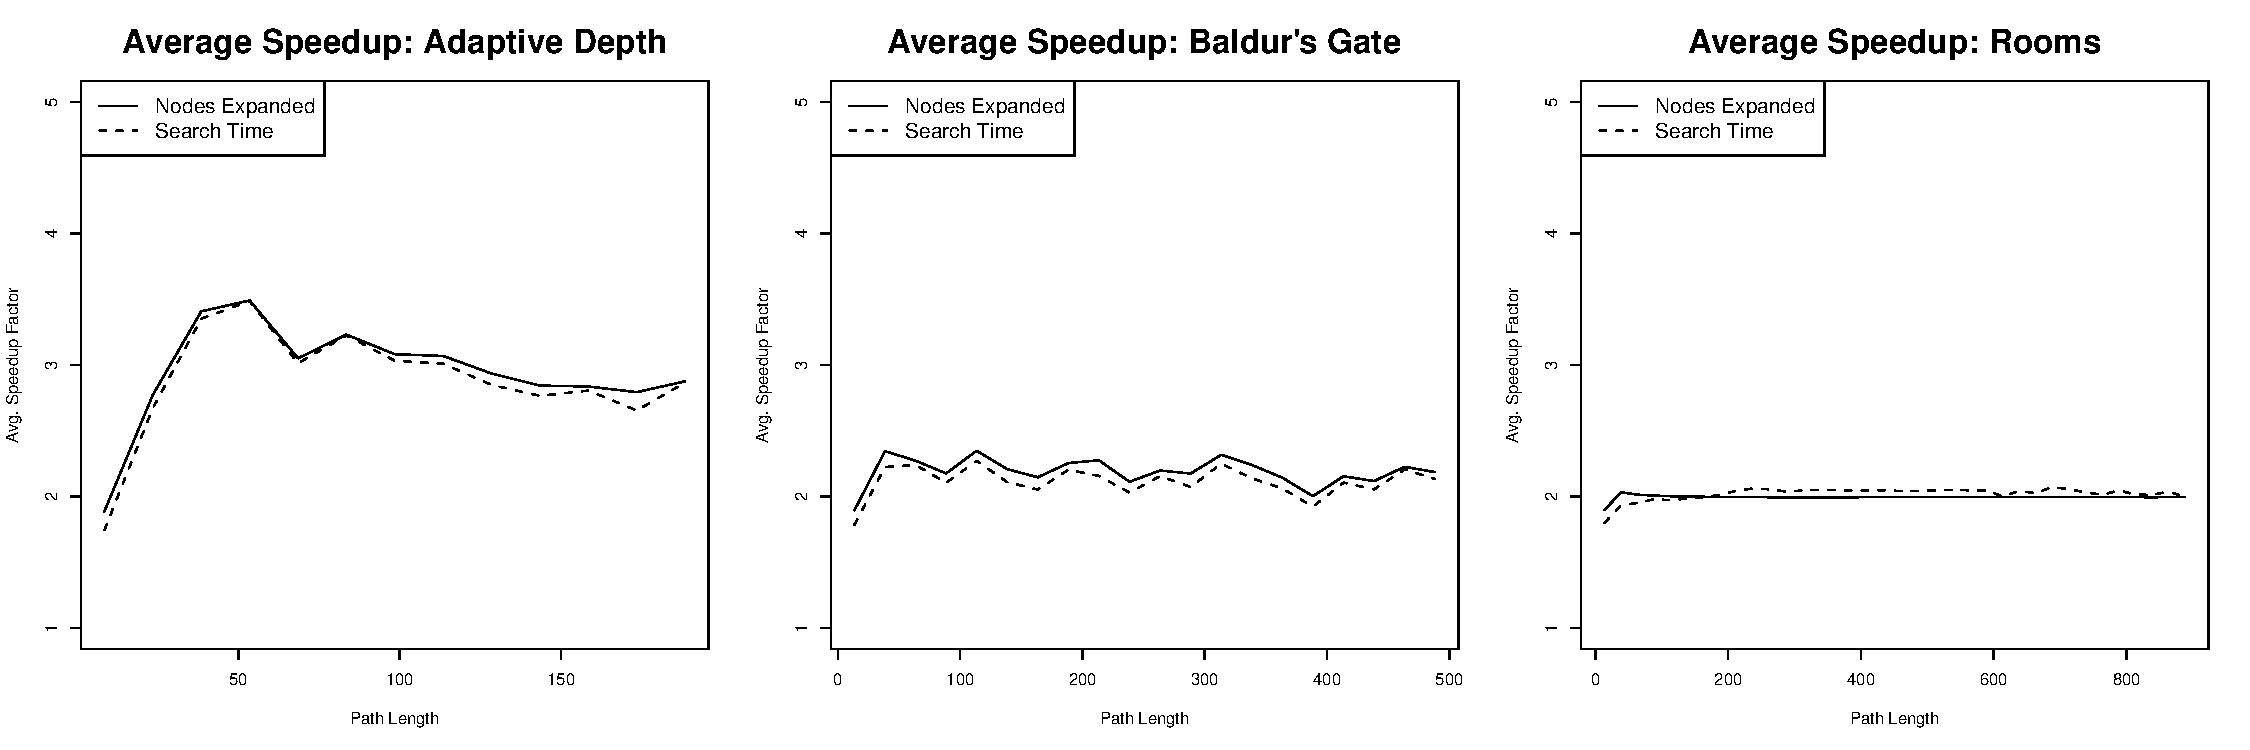
\includegraphics[width=0.95\columnwidth, trim=10mm 0mm 10mm 0mm]{diagrams/speedup.pdf}
\caption{Performance of our new algorithm on a range of benchmarks -- including one from BioWare's popular roleplaying
game \emph{Baldur's Gate.}}
\end{center}
\end{figure}
